\problemname{Järnvägen}

I dessa tider av avreglerad järnväg bestämmer sig Loke för att starta ett eget tågföretag som ska trafikera en viss järnvägslinje. Längs denna järnväg finns flera stationer och ett av Lokes första projekt är att bestämma vid vilka stationer det viktiga morgontåget ska stanna. Loke vill grunda sitt beslut på en stor enkätundersökning där han frågat varje tänkbar resenär mellan vilka stationer de vill åka och hur lång restid de kan tänka sig innan de väljer något annat färdsätt. Skriv ett program som utifrån detta underlag bestämmer vilka stationer tåget ska stanna vid för att det totala antalet personkilometer ska bli så stort som möjligt.

\begin{figure}[!h]
\begin{center}
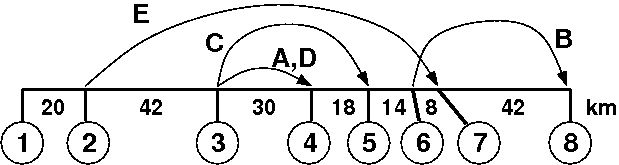
\includegraphics[width=0.7\textwidth]{jarnvagen.png}
\end{center}
\caption{Järnvägen i exemplet. Pilarna visar personernas önskade ressträckor. Beroende på vilken maximal restid E väljer så blir olika mellanstationer optimala. I exempel 1 åker A, B, C och D med tåget. I exempel 2 åker B och E. I exempel 3 åker A, D och E. I exempel 4 åker A, B, D och E.}
\label{fig1}
\end{figure}

\section*{Indata}

På första raden står två heltal $3\le N\ \le 20$, antalet stationer, och $1 \le P \le 100$, antalet tillfrågade personer. Stationerna är numrerade i ordning längs spåret från startstationen 1 till slutstationen $N$ (vid dessa två stationer måste tåget givetvis stanna). Därefter följer en rad med $N-1$ heltal i intervallet 2 till 1000, längden i kilometer på varje delsträcka mellan stationerna (se figur). Samtliga dessa tal är för enkelhets skull jämnt delbara med två. Tåget går nämligen normalt alltid med 120 km/h hastighet, d.v.s. varje kilometer tar exakt en halv minut. Inbromsning och acceleration gör dock att tiden för varje delsträcka förlängs med en minut om tåget stannar vid en av stationerna i delsträckans ändpunkter och två minuter om det stannar vid båda stationerna. Ingen extra tid behöver räknas för in- och avlastning, utan ankomsttid och avgångstid är samma. Slutligen följer $P$ rader med enkätsvaren, där varje rad innehåller svaren från en person: tre heltal $A$, $B$ och $M$, där $A$ är stationen personen vill åka från, $B$ är stationen personen vill åka till och $M$ är den maximala restiden (i minuter) han eller hon kan tänka sig. Talen uppfyller $1\le A < B \le N$, samt $2\le M\le 1000$.

{\bf Delpoäng:} För 30\%\ av poängen gäller att $N \le 10$.

\section*{Utdata}

Första raden ska innehålla det maximala antalet personkilometer som kan tillryggaläggas, d.v.s. för varje passagerare som får sina krav tillgodosedda summerar man sträckan som hon eller han reser. Sedan ska programmet skriva ut tidtabellen som åstadkommer detta maximala antal personkilometer. Den består av en rad med två tal för varje station som tåget stannar vid: stationens nummer samt tidpunkten då tåget stannar där. Tåget startar alltid vid tiden 0. Om det finns flera möjliga tidtabeller ska programmet välja en som är framme vid slutstationen så tidigt som möjligt.

